\section{Waffle}
\label{sec:3-instr}

% Done: The key idea is that I should talk about my solution to the program with more details.
% Done: I have explained that there is another way of resolving the problem.
% Now it's time to explain what is the difference in the guidance defined in Waffle
% Definitions?!:
% Resource complexity, Overall resource complexity (ORC), Elites, Visitors
% OR: Shared memory, instrumentation, fuzzing

% How does the new features solve the problem?
% ! Change Instruction to Machine Instruction

% Tasks
% -T1: Explain the way AFL works
% -T2: Explain an overview of the additional properties added to AFL by Waffle
% Keywords 
% -K1: exploration vs exploitation
% -K2: performance-guided fuzzing vs coverage-guided fuzzing

The exponential search space for different inputs with a specific behavior, such as a crash or hang, is approached by evolutionary algorithms of AFL to investigate the possible solutions for producing such events. AFL leverages on code coverage, file size, and execution time to guide the Genetic Algorithm to maintain the cases which discover more regions of the code, in a fast fasion. Waffle \textit{exploits} the coverage-guided findings for more resource usages. The key idea is to measure the performance in an execution, and provide this information in fuzzing phase to generate resource exhaustive inputs. 

% Tasks
% -T: Explain the waffle-proc.png

As illustrated in Figure \ref{fig:waffle-phases}, Waffle has major modifications on AFL in instrumentation phase (shared memory allocation and instructions insertion) and fuzzing phase. The shared memory is designed to be capable of storing the \textit{resource complexity} of an execution. Waffle also extends AFL's Coverage Pass to collect performance features as well. In the fuzzing phase, Waffle evaluates the code coverage and resource usage of the execution, and based on this information culls the queue of entries to consider the new performance measurements. In the following sections we inspect the changes and assess the effectiveness of the work.

\begin{figure}[!b]
  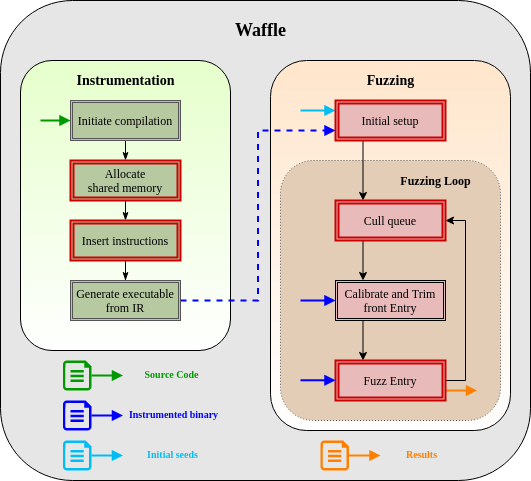
\includegraphics[width=0.8\textwidth]{Chapter3/waffle-proc.png}
  \centering
  \caption{Fuzzing phases of Waffle. The red rectangles specify the changed components.}
  \label{fig:waffle-phases}
\end{figure}

\subsection{Resource complexity of execution}

% Tasks
% -T: What the resource complexity is and how it is measured

To address resource usage of an execution, we estimate the engaged resources in an execution. Waffle does not analyse the source code for finding the resource complexities, such as time and space complexity, however, it records the instructions responsible for resource consumptions. For instance, an instruction such as \texttt{memcpy} takes CPU usage (and time) for its execution, and may access the program's available memory. To bring in the involved instructions in a complete run of a program, Waffle selects a set of instructions and monitors the program's execution of such instructions. The accumulation of the executed instructions is then stored partially in the shared memory.

% Tasks
% -T1: Estimated Resource Usage

We define the \textbf{Estimated Resource Usage} (shortened to ERU) of an application for \textit{an estimation of the resources required to execute a program}. To evaluate the ERU of a program in a concrete execution, each instruction which uses the \textit{engaging resources} should be monitored. For instance, an instruction such as \texttt{memcpy} takes CPU usage for its execution, and may access the program's available memory.  

% Tasks
% -T1: How waffle uses the ERU through entire fuzzing chain

Waffle replicates AFL's coverage-discovery techniques with modifications to calculate and leverage ERU for performance-guidance. Waffle selects a set of instructions and counts their executions to get ERU. The ERU is then stored in an array of the same size as the AFL's coverage map, and for each hit on the coverage map, Waffle changes the same index of it's performance array. As a result, the hitmaps of both of the arrays are the same, and they both can represent the code-coverage; each index is found based on the taken edge of the CFG. Later, in the fuzzing phase, Waffle uses ERU to choose the \textit{favored} entries of queue. In AFL, a favored entry is relates to the input which brings something new, that is, a better code coverage or a faster execution. Instead, Waffle finds the \textit{favor} in any entry which is either AFL-guided or Waffle-guided; a better code coverage or a more exhaustive execution.

% !     Subsection 1: Instrumentation
\subsection{Instrumentation}
\label{subsec:inst}

% Tasks
% -T1: Generally define and explain the added and modified modules in Instrumentation

Waffle starts its instrumentation by specifying the shared memory region. Waffle maintains an array of 4bytes integers for tracking the ERU of each basic block. This array's length is the same as the AFL's shared array, and as a result, the Waffle's array requires 4x more memory space (Listing \ref{lst:wafl-rt}). This array is set to hold the counts of the edges according to the paths explored. When the initial setups are completed, the next instrumentation step, taking the Module Pass starts.
  
\lstinputlisting[language=C,style=CodeStyle,float=tb,label={lst:wafl-rt},caption={LLVM instrumentation initialization - \texttt{\_\_wafl\_area\_ptr} is the region that is allocated for instruction counters}]{Codes/Chapter3/waffle-llvm-rt.o.c}  


% Tasks:
% -T1: Explain LLVM visitor functions
% -T2: Explain the implementation of the visitor functions

% \subsubsection{Visitors}

Waffle uses \textit{LLVM's instruction visitor functions} \cite{inst_visitor} to investigate and count engaging features in the machine code. LLVM provides functions for \texttt{getting} and \texttt{setting} the instructions in a range of address in the code section of the program. This API is applied on the IR of the program and Waffle uses it in the Module Pass of the compilation. Listing \ref{lst:visitors} shows an example of how Waffle implements the counters for instructions; the member function \texttt{visitInstruction(Instruction \&I)} checks if the instruction is of \textbf{any} type, and as a result, an instance of the class \texttt{CountAllVisitor} can contain the occurences of (any) instructions in a range of instruction pointers.

\lstinputlisting[language=C++,style=CodeStyle,label={lst:visitors},caption={Visitors example}]{Codes/Chapter2/visitor.cpp}

% TODO: Probably explain another example for the counters, like the one checking the memory activities. 
% * Future work: Using different visitor classes? 

A snippet of the Module Pass is shown in Listing \ref{lst:llvm-pass}. In line 6 the pointer to the shared array is introduced; Lines 10 to 14 includes the previously defined function for sum of ORCs, \texttt{addORC()}. After the initial set up, Waffle digs into the basic blocks and create and instance of the \texttt{CountAllVisitor} struct. By passing the current basic block to the visitor, the visitation of EI is stored in \texttt{CAV}. The linear increment in \texttt{CAV} has a relatively large variance in effectiveness of each basic block in changing the total ORC. For instance, if Waffle chooses to count all instructions in the execution, the basic blocks contributed an average of $18$ instructions for the ORC \footnote{Tested C++ implementations of QuickSort, MergeSort, and DFS}. To reduce the impact of large numbers in ORC, Waffle calculates the logarithm of the each counter: 

\begin{equation}
  \label{eq:log}
  CNT = \log_{2}^{CAV+1} 
\end{equation}

The EI-ORC of a basic block is then prepared for storage in both of the storages. Waffle inserts instructions for loading the according index in the shared memory, adds the reduced estimation of EI-ORC to the loaded value, and stores the result back in the same index. Finally, Waffle adds \texttt{CNT} to the \texttt{total\_ORC} by calling the function \texttt{addORC} (Line 42).

\lstinputlisting[language=C,style=CodeStyle,label={lst:llvm-pass},caption={LLVM-mode instrumentation pass}]{Codes/Chapter3/mini-wafl-llvm-pass.so.cc}

Waffle builds its own compiler using the above definitions in instrumentation stage. By making (compiling) the files in \texttt{llvm-mode} directory, an executable compiler, \texttt{waffle-clang} is generated. This compiler scans the source code of the program, and creates a binary file with the logic of the program, and the intended instrumentation:

\begin{lstlisting}[language=bash,style=CommandStyle,label={lst:wafl-clang}]
  ./waffle-clang target.c -o instr_target.bin
\end{lstlisting}